%!TEX root = ../thesis.tex
\chapter{Coregistration of High Resolution Rat Histology}
% If you like chapter abstracts ...
\dblspace
\begin{quote}{\em %!TEX root = ../thesis.tex
Adjacent histological slices can be coregistered accurately and lead to smooth image volumes, owing to their close morphological resemblance and their similar intensity spectra. However, volumes constructed from serial histology registration do not reflect the true 3-dimensional tissue geometry. Registration of histology to a set of coherent reference images yields an authentic geometry on the organ scale, yet the lower resolution and differing modality of the references leads to noisy, jagged volumes on the microstructural scale.

We present in this chapter an algorithm to align neighbouring slices accurately and smoothly without disturbing large scale tissue shape, based on a microscopic model of diffusion. We develop a mathematically sound and general framework of transformational diffusion, based on the Lie theory of continous groups. Using synthetic geometries of cardiac tissue with artificial noise, we demonstrate a robust and precise dispersion of information between slices on a configurable range of scales, recovering volumes which are orders of magnitude smoother and which have maintained faithfully the underlying geometrical signal. We apply the algorithm to the volumes from Chapter~\ref{cha:coregistration_of_high_resolution_rat_histology}, first globally and then again to the region around an epicardial vessel. Previously indiscernible microvasculature and sheet structure become patent. Pericardium and epicardial vessel segmentations show that displacement abberations between adjacent slices of the order of 400$\mu$m are reduced by two orders of magnitude. The methods presented here outperform any such method to reconstruct histological volumes based on reference images currently in the literature. Finally, we discuss several interesting applications and refinements that might be made to the algorithm in specific cases, including anisotropic diffusion based on image features or inter-slice transform magnitudes. The results of this work are presented Computational Methods in Systems Biology 2012 \cite{Gibb2012}, and the work in Chapter~\ref{cha:coregistration_of_high_resolution_rat_histology} and this Chapter will be published in detail in IEEE Transactions on Medical Imaging.
}\end{quote}

CONFIRMATION REPORT
\section{Aims}
  MOTIVATION, PROBLEMS, AIMS
  
  Intro/Motivation
  People have tried to align block faces, but can't use certain dyes, transmission problems, lo res with Lo res data.
  People have tried to align hires stuff, but we know that this is not consistent.
  ASK VICENTE FOR REFS. MARK BOYETT FIRST AUTHOR OF ONE PAPER. ASK BECKY FOR INTRO/METHODS PAPERS.
  First attempt to use both sets of data to make coherent hires dyed segmented etc.
  
  The aim of this chapter is to develop an automated pipeline to register high resolution rat cardiac datasets robustly and accurately, and generate coherent subcellular resolution 3-D cardiac histological images.  Approximately three full rat heart datasets will be processed through the pipeline to provide registered volumes. These images will serve both as an authoritative anatomical reference, and as the basis for anatomically based models in simulation studies.

\section{Methods} % (fold)

PROGRESS FROM CONFIRMATION REPORT 
An iterative 2D-3D registration pipeline has been developed for registering rabbit histology images to their associated MRI volume. Since transfer, it has been made clear that the precision of registration required to extract fibre direction far exceeds that which could be achieved with the iterative method. New rat data has become available with two sets of 2D images: a high resolution unregistered histological slice and a related lower resolution image of the surface of the embedded heart block before each slice is cut. The coherent set of wax block images vastly simplify the problem and facilitate far more accurate results.

END PROGRESS FROM CONFIRMATION REPORT 



\label{sec:methods}
  Basic structure of methods section
  
  \subsection{Image Preparation and Curation} % (fold)
  \label{sub:image_preparation_and_curation}
    \begin{sidewaysfigure}[htbp]
      \centering
      \subfigure[][]{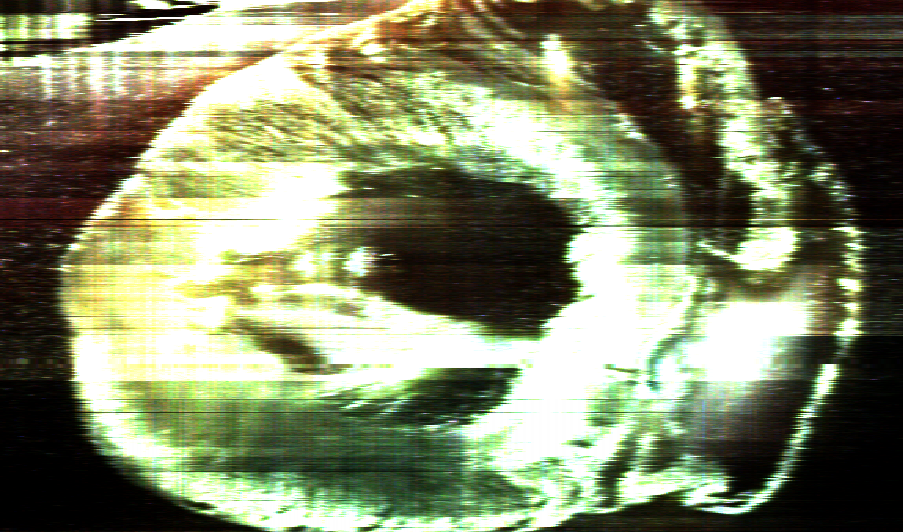
\includegraphics[height=0.31\textheight]{Ch6/Figs/LoRes_0_235}}
      \subfigure[][]{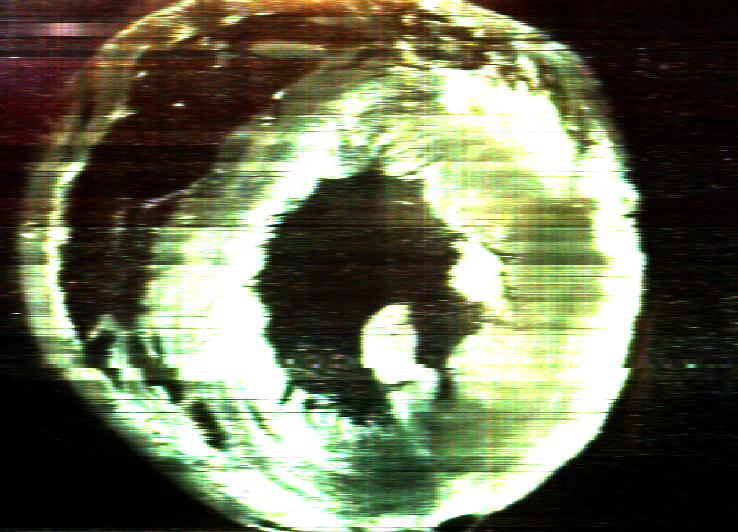
\includegraphics[height=0.31\textheight]{Ch6/Figs/LoRes_1_287}}
      \subfigure[][]{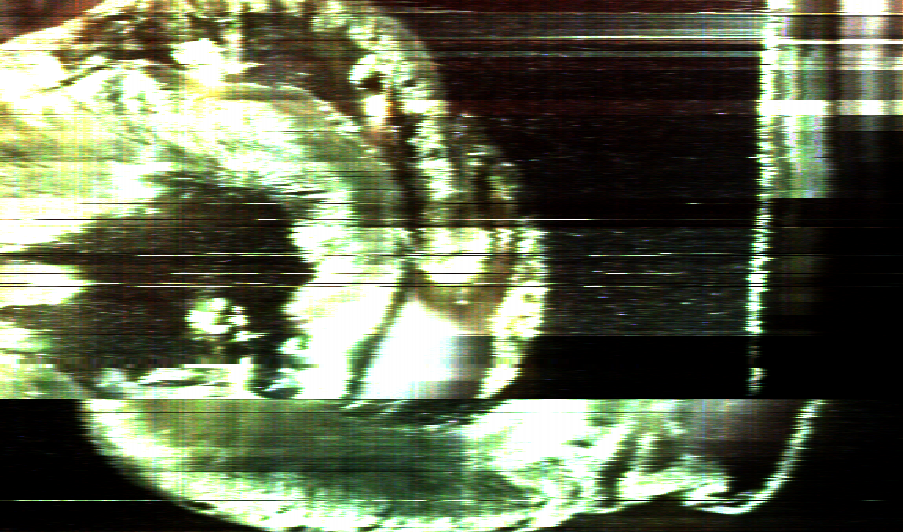
\includegraphics[height=0.31\textheight]{Ch6/Figs/LoRes_without_adjustments_0_235}}
      \subfigure[][]{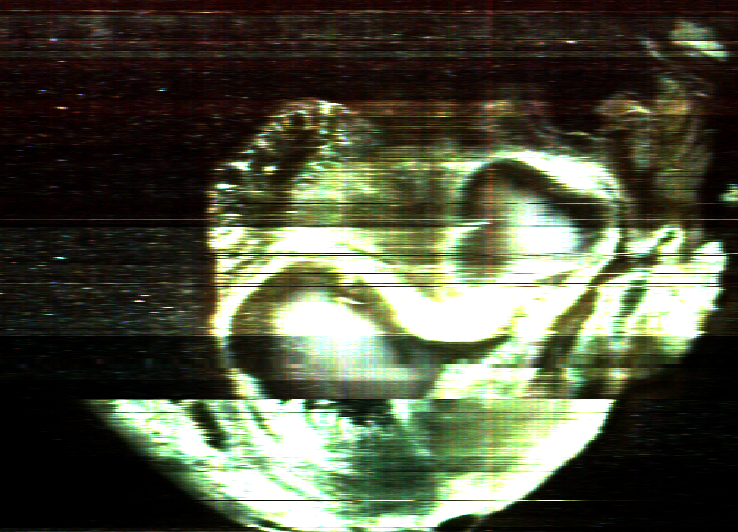
\includegraphics[height=0.31\textheight]{Ch6/Figs/LoRes_without_adjustments_1_287}}
      \caption{What a nice figure!}
      \label{fig:LoRes_cross_sections}
    \end{sidewaysfigure}
    
    Figure of single LoRes slice with equivalent HiRes slice
    \begin{figure}[htbp]
      \centering
      \subfigure[][]{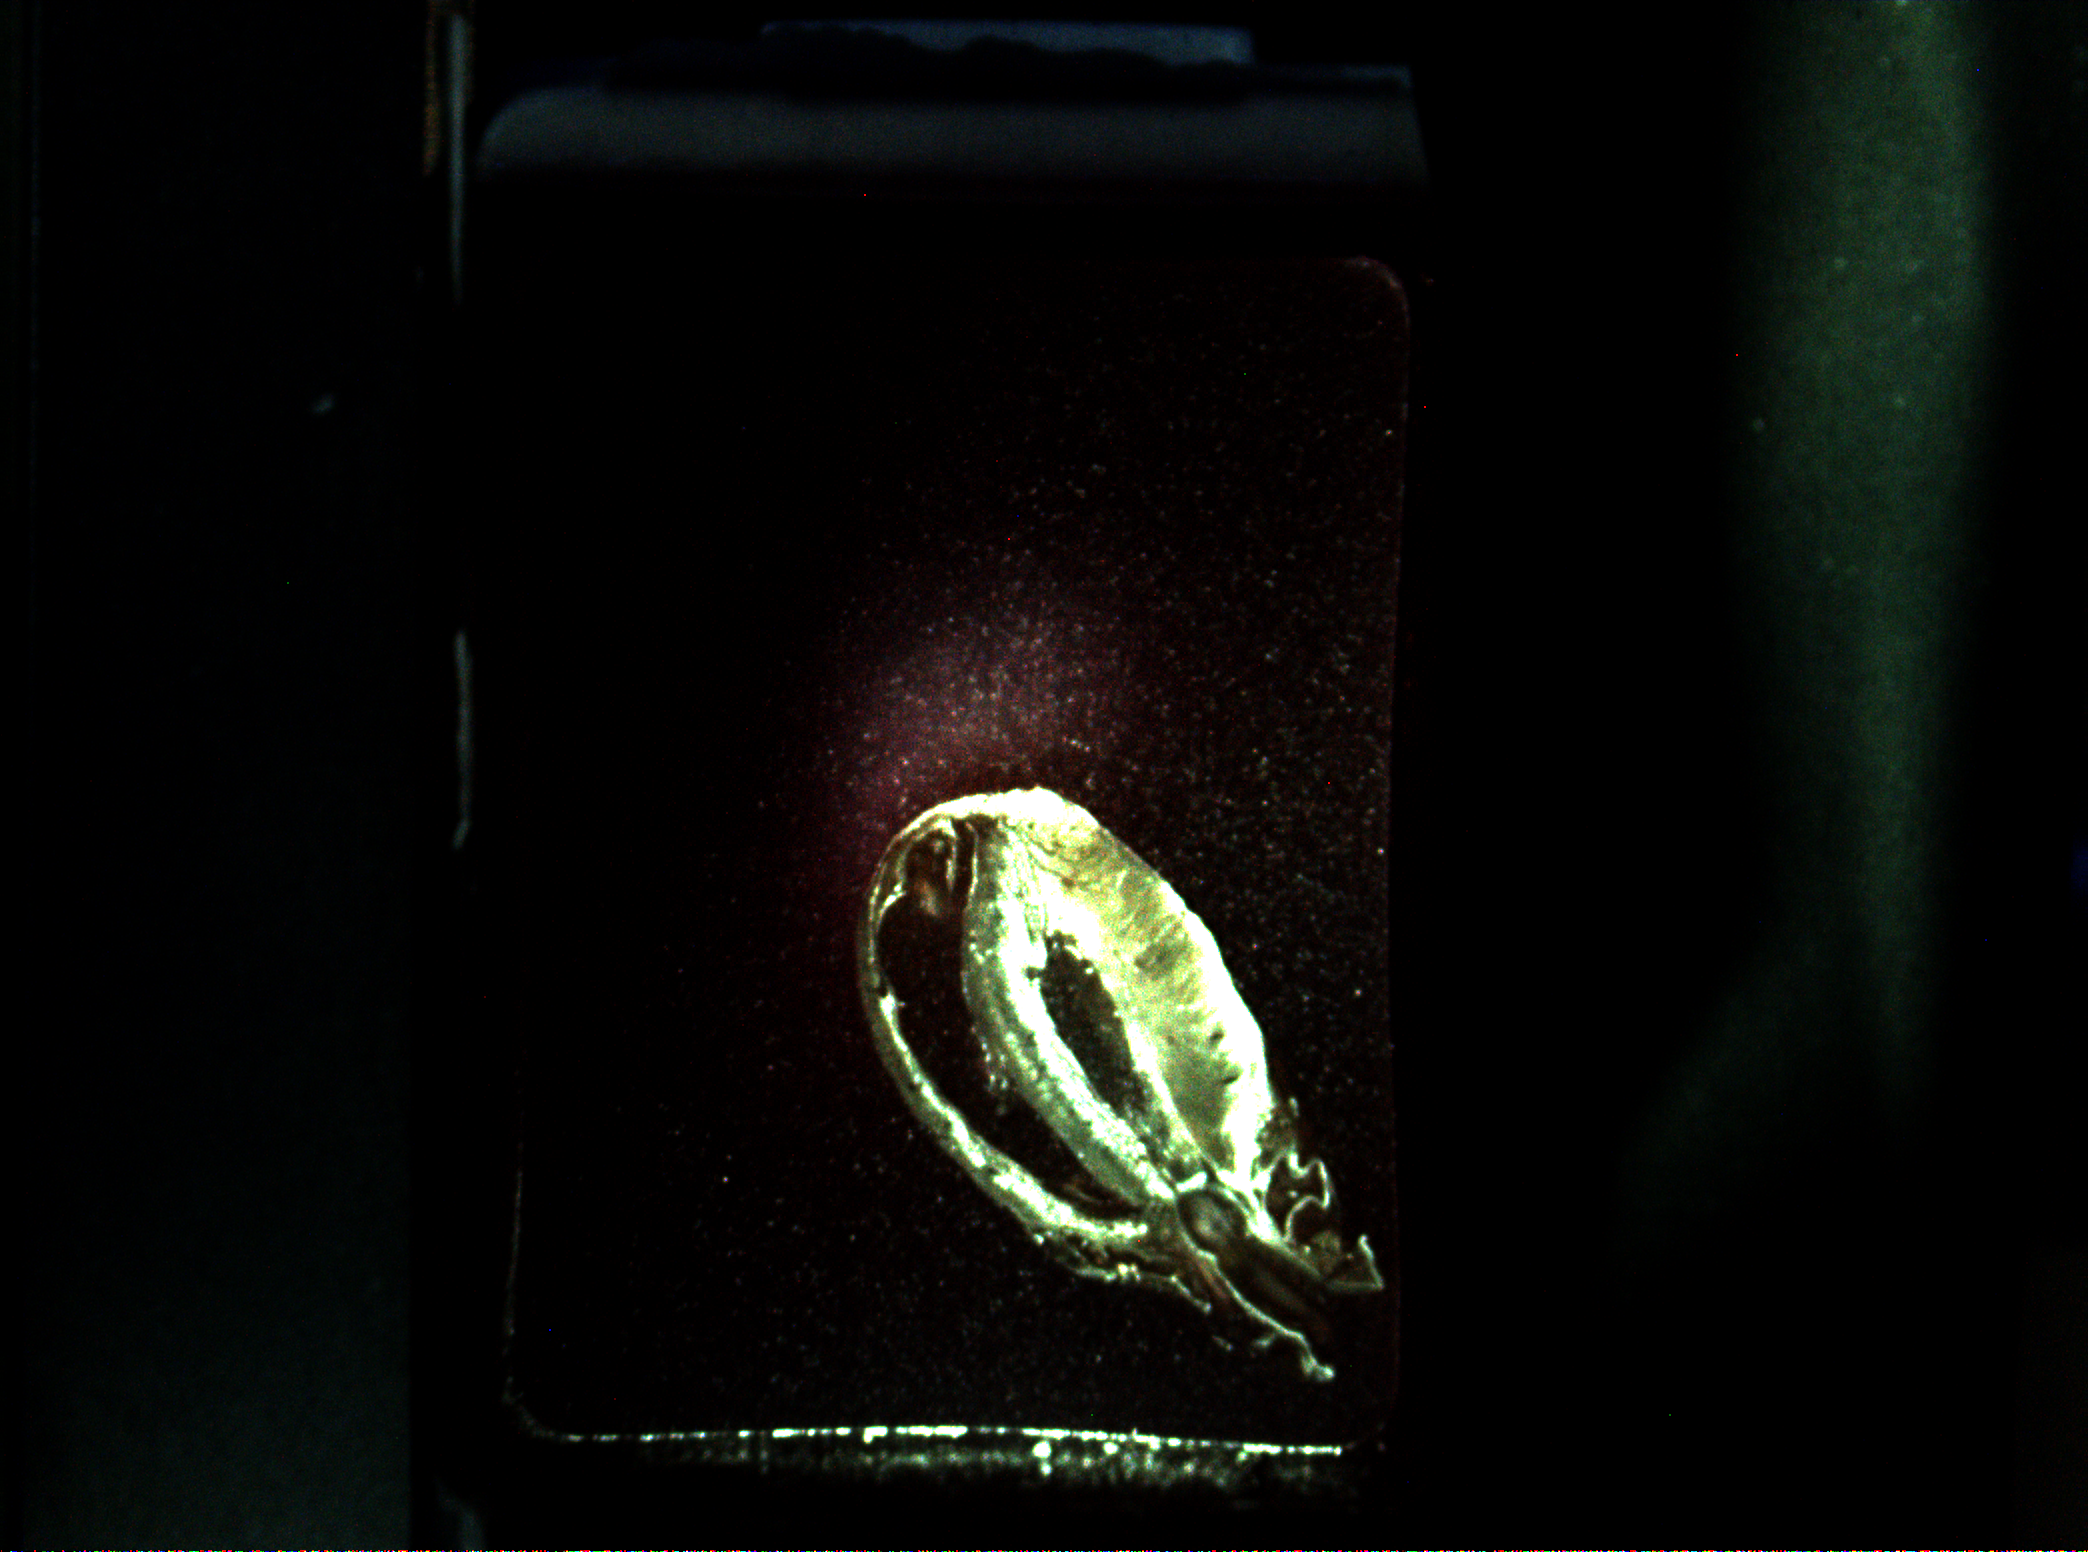
\includegraphics[width=0.4\pagewidth]{Ch6/Figs/LoRes_rgb_downsamples_1_0582}}
      \subfigure[][]{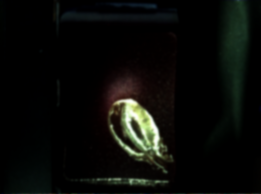
\includegraphics[width=0.4\pagewidth]{Ch6/Figs/LoRes_rgb_downsamples_8_0582}}
      \caption{}
      \label{fig:original_images}
    \end{figure}
    
    \begin{figure}[htbp]
      \centering
      \subfigure[][]{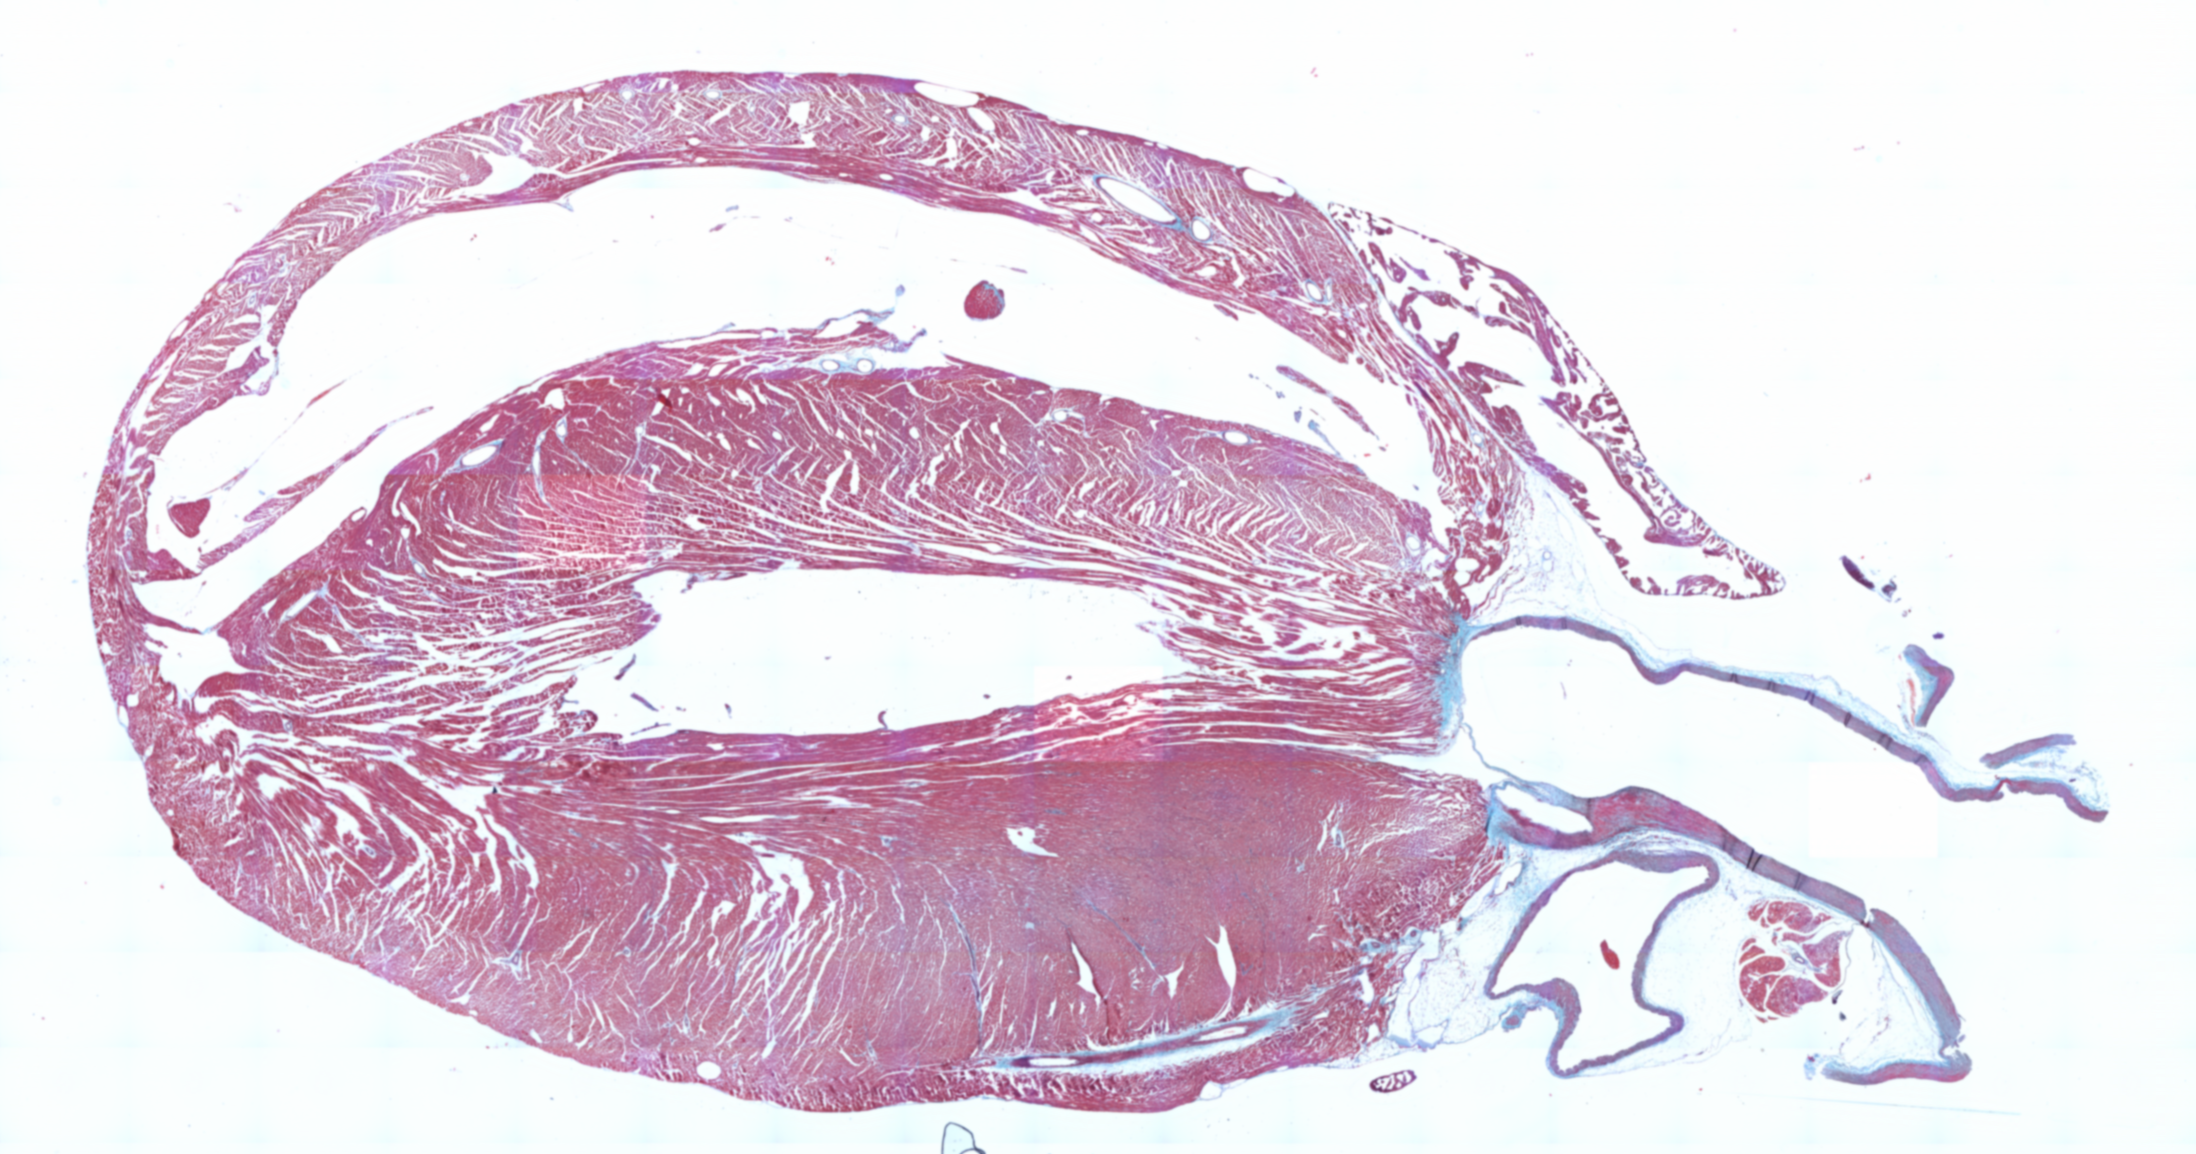
\includegraphics[width=0.4\pagewidth]{Ch6/Figs/HiRes_downsamples_8_0582}}
      \subfigure[][]{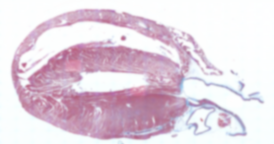
\includegraphics[width=0.4\pagewidth]{Ch6/Figs/HiRes_downsamples_64_0582}}
      \caption{Mention how the slice needs to be flipped and rotated to be in line with the block face image.}
      \label{fig:original_images}
    \end{figure}
    
    \begin{sidewaysfigure}[htbp]
      \centering
      \subfigure[][]{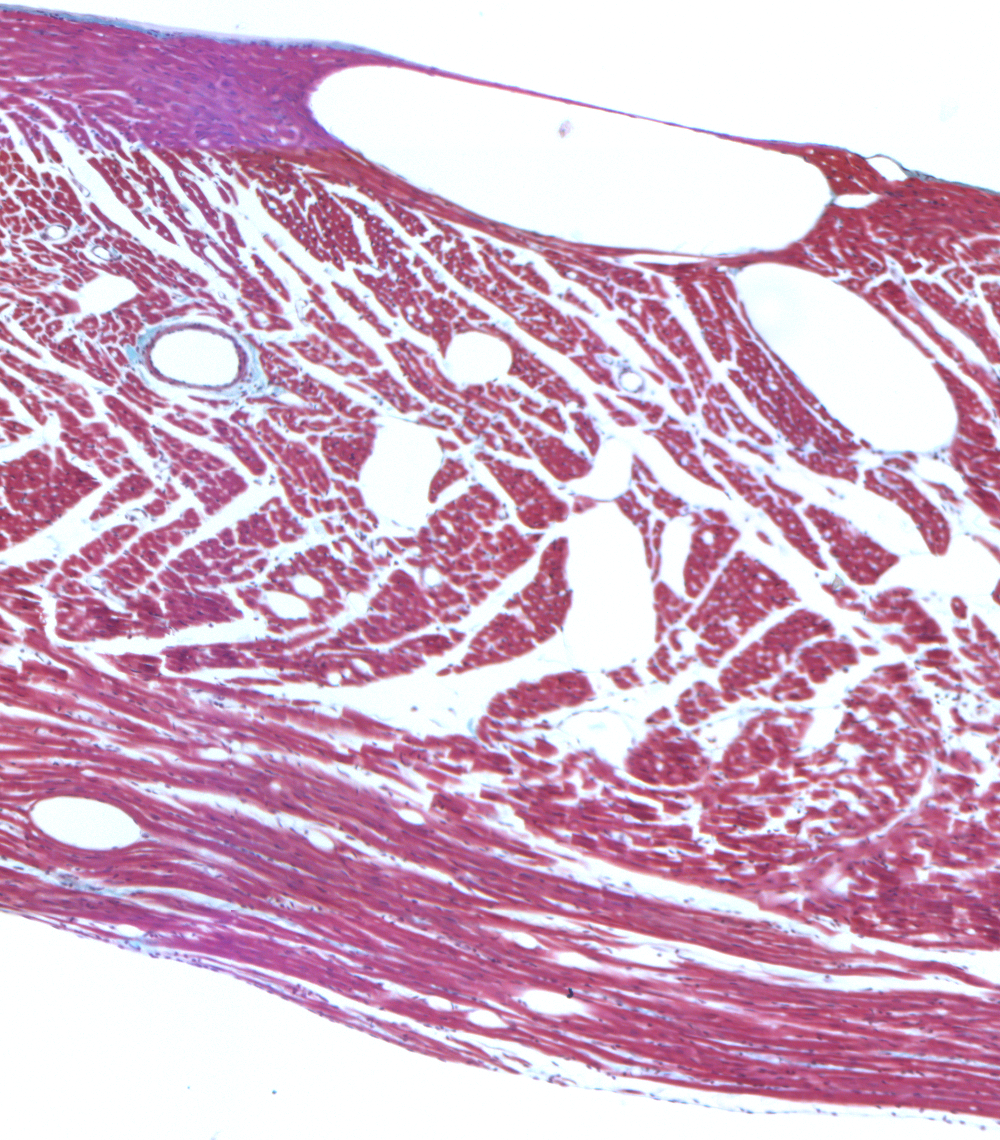
\includegraphics[width=0.4\pagewidth]{Ch6/Figs/HiRes_downsamples_1_0582_zoom}}
      \subfigure[][]{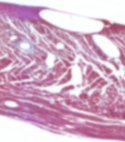
\includegraphics[width=0.4\pagewidth]{Ch6/Figs/HiRes_downsamples_8_0582_zoom}}
      \subfigure[][]{
\includegraphics[width=0.4\pagewidth]{Ch6/Figs/HiRes_downsamples_64_0582_zoom}}
      \subfigure[][]{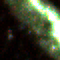
\includegraphics[width=0.4\pagewidth]{Ch6/Figs/LoRes_rgb_downsamples_1_0582_zoom}}
      \subfigure[][]{
\includegraphics[width=0.4\pagewidth]{Ch6/Figs/LoRes_rgb_downsamples_8_0582_zoom}}
      \caption{Mention how the slice needs to be flipped and rotated to be in line with the block face image.}
      \label{fig:original_images}
    \end{sidewaysfigure}
    
    downsampling, RGBA, flipping and rotating, a few figures
    
    LoRes adjustments:
    Figure of full LoRes volume without and with adjustment, with 1 quarter cutaway
    
  % subsection image_preparation_and_curation (end)
  
  \subsection{Initialisation} % (fold)
  \label{sub:initialisation}
    Motivational paragraph: registration is sensitive to starting params, prone to trap into local minima...
      
    Slice images were flipped and rotated to align approximately with the block images. 
    
    
    White space under the microscope surrounding the slices had already been cropped, such that each slice sat approximately central within the bounds of its image. Thusly, slice images were aligned to their common geometric centre.
    
    Figure: A naive initialisation of the histological slices, aligning images to their common centre, provides an adequate starting point. VOLUMES ALONG WITH MASKS
    Figure: Cutthroughs and volume with quarter missings of HiRes images before registration
    % Possible figure: 3/4 volume of image mask to demonstrate geometric centres
    
    The initial translation and pixel spacing of the LoRes images were manually tuned to overlap maximally with the HiRes data set.
    
  fig
    
  % subsection initialisation (end)
  
  \subsection{Rigid Registration} % (fold)
  \label{sub:rigid_registration}
    By far most of the registration is done in the first rigid step. Didn't work for lots of reasons, tried PCA, ITKv3 bug, different metrics, optimisers, normalising images etc. loads of figures.
  % subsection rigid_registration (end)
  
  \subsection{Similarity and Affine Registrations} % (fold)
  \label{sub:similarity_and_affine_registrations}
    Show instabilities and scaling factor problems
    
    further non rigid?
  % subsection similarity_and_affine_registrations (end)
  
  \subsection{Multiresolution Registration} % (fold)
  \label{sub:multiresolution_registration}
    Multires was tried. Discuss proposed advantages: faster, smoother cost function...
  % subsection multiresolution_registration (end)
  
  \begin{figure}[htbp]
    \centering
    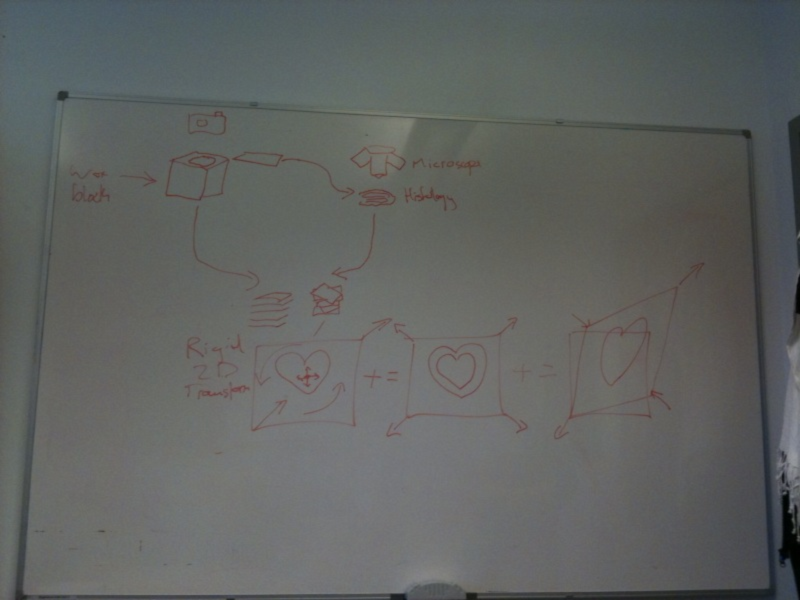
\includegraphics[height=0.7\textwidth]{Ch6/Figs/process_diagram}
    \caption{A schematic of what's going on.}
  \end{figure}
  
  Each rat heart was embedded in black wax and serially sliced. For each rat heart, two complimentary datasets have been provided: one of the top surface of the wax block before each slice, and one high resolution image of the rehydrated slice under microscope. The block images are not subject to individual deformations and thus form a coherent 3D data set. The challenge is thus to register the slices with their equivalent block face images in 2-D.
  
  The images are downsampled and preprocessed using one of a number of intensity rescaling schemes. Registrations are performed in an iterative fashion, gradually reducing in transformation constraint, starting with a simple rigid transform. Finally, a series of non-rigid bspline registrations are performed at progressively higher resolutions.
   
    \subsection{Diagnostics} % (fold)
    \label{sub:diagnostics}
      For a year and a half, very difficult to see why registration was failing. Output of raw parameters got us somewhere, but only for obvious issues e.g. parameter scaling, step length. Huge parameter space. Sports game analogy about result, but no play-by-play. BuildProgressVolumes
      
      Parameter tuning:
      
      Figures of bad params, symptoms and results. e.g. zigzags, overshoot and gradual worsening. Unclear how the gradual worsening happens; could be an oddly shaped v-shaped cost basin, deepening steeply along one dimension and 
      
      Before upgrade to ITKv4, registration algorithm would often not optimise i.e. results were much worse. Even though the upgrade shouldn't have affected the results, just the speed of the code, results were much much better.
      
      Parameter tuning:
      Initial discussion of 4 parameters in RSGD: 2 behavioural (max step and relaxation factor), and 2 cutoff(min step and gradient magnitude tolerance).
      Figures need to compare:
        increase/decrease in behavioural (zigzag if too high because of overshoot)
      increase/decrease in cutoff (takes too long if low, see tails in plot metric values and differences, doesn't finish if too high, use compare final metric values.py)

      Increase max step for HiRes pairs registration to 60, and show characteristic zigzagging and jumping out of potential well

      
    % subsection diagnostics (end)
% section methods (end)
   
\section{Results}
  A series of figures will provide visual validation of the results, both of the full heart and more detailed images in regions of interest. Cross-sectional images perpendicular to the slice planes will show the close matching between planes, and segmented surfaces of myocardial walls and larger arteries will be rendered in 3-D. The performance of various registration regimes will be compared.
CONFIRMATION REPORT

% initialisation figure
\begin{sidewaysfigure}[htbp]
  \centering
  \subfigure[][]{
\includegraphics[height=0.31\textheight]{Ch6/Figs/geometric_0_235}}
  \subfigure[][]{
\includegraphics[height=0.31\textheight]{Ch6/Figs/geometric_1_287}}
  \caption{}
  \label{fig:hires_0_235}
\end{sidewaysfigure}

% x slices
\begin{figure}[htbp]
  \centering
  \subfigure[][]{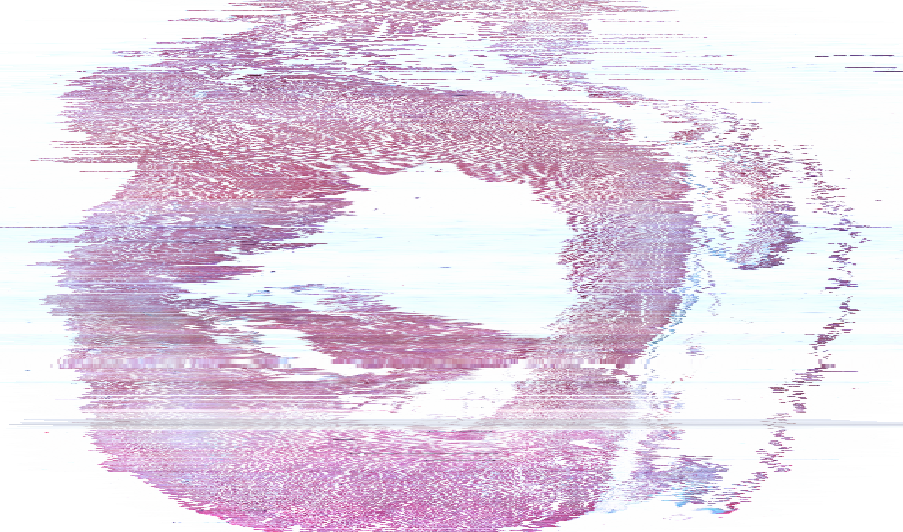
\includegraphics[height=0.31\textheight]{Ch6/Figs/rigid_0_235}}
  \subfigure[][]{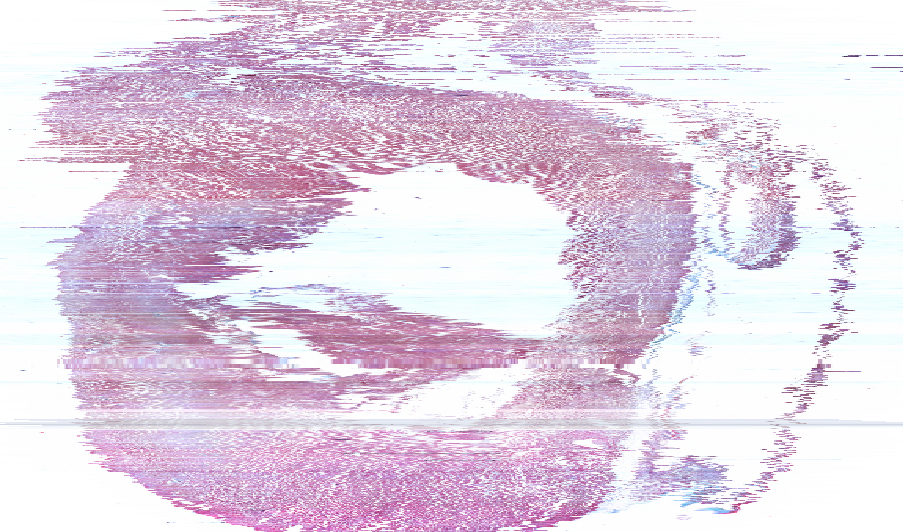
\includegraphics[height=0.31\textheight]{Ch6/Figs/size_0_235}}
  \subfigure[][]{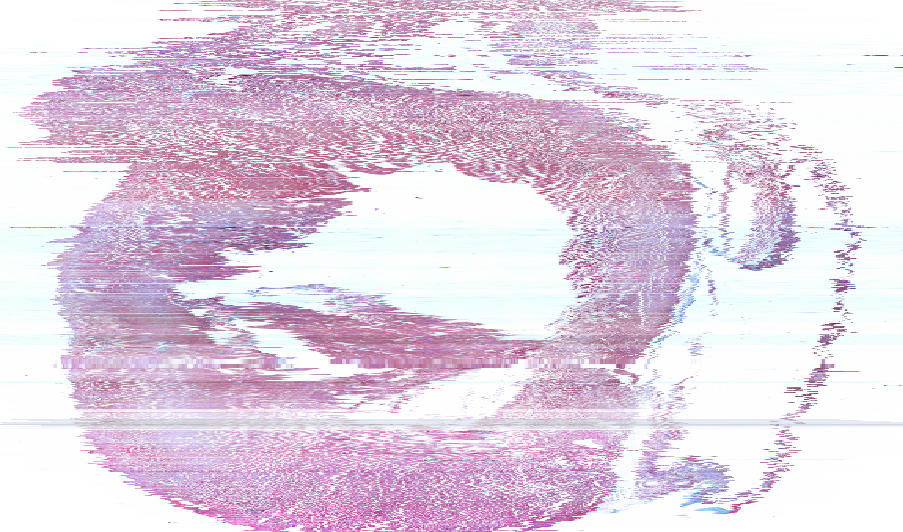
\includegraphics[height=0.31\textheight]{Ch6/Figs/affine_0_235}}
  \caption{Talk about how discontinuities in intensity between slices in the LoRes cutthrough fig are mirrored in the registration}
  \label{fig:hires_0_235}
\end{figure}

% y slices
\begin{figure}[htbp]
  \centering
  \subfigure[][]{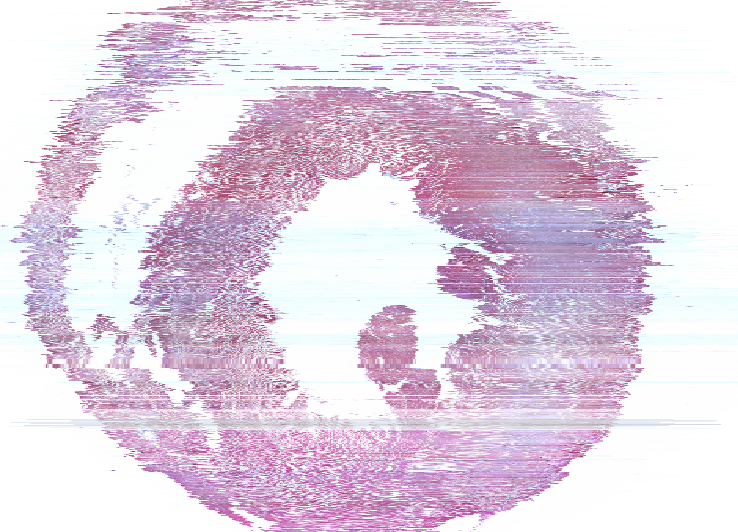
\includegraphics[height=0.31\textheight]{Ch6/Figs/rigid_1_287}}
  \subfigure[][]{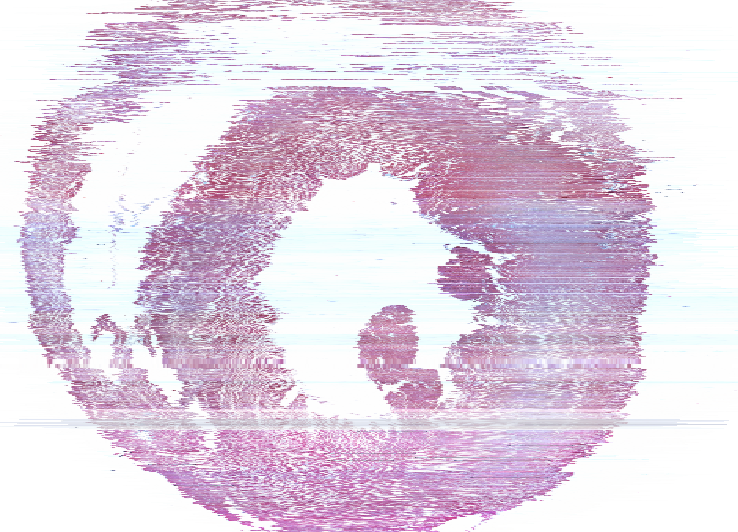
\includegraphics[height=0.31\textheight]{Ch6/Figs/size_1_287}}
  \subfigure[][]{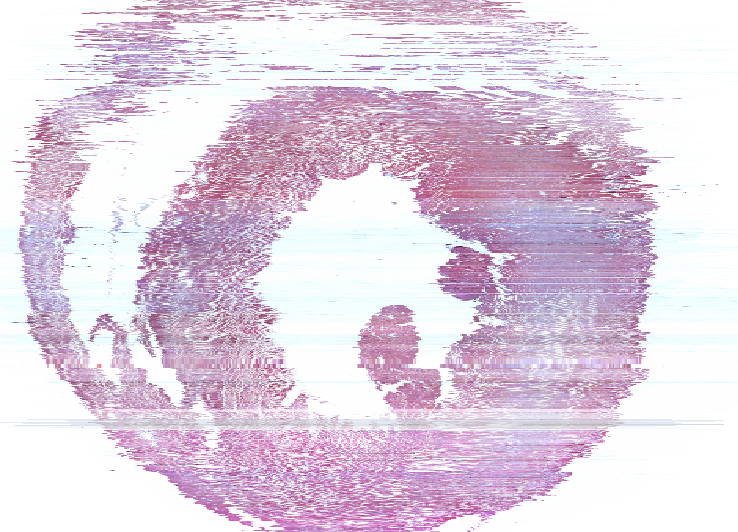
\includegraphics[height=0.31\textheight]{Ch6/Figs/affine_1_287}}
  \caption{What a nice figure!}
  \label{fig:hires_1_287}
\end{figure}

\section{Evaluation} % (fold)
\label{sec:evaluation}

\textit{PROGRESS FROM CONFIRMATION REPORT 
A full-heart registration pipeline has been developed and downsampled histological volumes generated. An initial manual alignment is followed by rigid and similarity transforms. The quality of the registrations are quite poor at present, and the task at hand is to fine-tune the various parameters that constrain the process: parameter space preconditioning, maximum iterations, maximum and minimum step lengths, number of spatial samples and metric-specific parameters.
END PROGRESS FROM CONFIRMATION REPORT
}

    Talk about ad hoc meta-optimisation of registration parameters, could be more formalised but a great deal more effort and prone to error (e.g. mean final metric values of all slices might decrease, but end result may suck)
    
    The method for optimising registration parameters is a crude and intuitive version of the optimisation algorithms applied to the image registrations. Not easily possible to calculate gradient of metric in parameter space, but can perturb coordinates along basis axes e.g. parameter scaling, choice of metric or optimiser, gradient descent learning rate, RSGD relaxation factor, whether to normalise images etc. 2 approaches: could split the space into two groups of `preferred' axes, and secondary axes, then perform an (exhaustive?) prototype search in the preferred subspace, and for each preferred coordinate perform an iterative optimisation in the secondary space. Alternatively, just perform iterative stochastic search in the whole space.
    
    ?NEEDS DEVELOPMENT? Some params like choice of metric have different associated parameter spaces e.g. learning rate vs relaxation factor, and also are likely to lead to widely different optimal spaces along other axes e.g. parameter scaling.
    
    Problems about things like histogram matching, Mutual info: for histogram matching there is no monotonic mapping between the intensity in the lores and that of the hires, with tissue /non tissue. With Mutual info, doesn't need to be monotonic, but there isn't even a one-to-one mapping i.e. many regions of tissue in lores occupy the same intensity range as non-tissue.

% section evaluation (end)

PAPER OUTLINE FROM CONFIRMATION REPORT
\subsection{Towards Coherent Subcellular Resolution 3D Cardiac Histological Images: Experimental and Computational Methods}
  This paper will be composed of four main sections: an overview of experimental methods, a review of the architecture of the library developed to register the raw data, a comparison of algorithms and their utility to this end, and finally the results of successful registration, with several colour figures providing visual validation of the methods.

  \subsubsection{Image Acquisition}
    This section will catalogue the preparation and imaging of the hearts: first the isolation from the rats, then the Langendorff perfusion and fixing, stabilisation in agar and MR scanning, and lastly the dehydration, wax embedding, sectioning and rehydration. Details and figures of both the wax block and the histological slice imaging processes will conclude this section.

    \subsubsection{Software Architecture}
      An outline of the main problems encountered during the development process will be exhibited, along with the solutions crafted to overcome them.
      
      \paragraph{Stacks}
        Histology data are provided in series of 2D png images. Images within a set can each be of unique size, and slices which were damaged or which have not been imaged yet are missing. Each block image must be paired with its equivalent slice image, and blank images must be interpolated where images are missing. Slices must be transformed independently and by a range of transforms. Binary masks must be generated for each image, so that metrics will only take pixel intensities into account from inside the boundaries of the original untransformed images. A minimum percentage overlap is required for many metrics to function, and for small slice images close to the apex of the heart, block mask areas must be cropped until this constraint is satisfied.
        
        The Stack has been developed to encapsulate the solutions to all of these problems. A Stack represents the 3D composition of a set of 2D slices. It handles ROI selection, generic transform storage, image and mask resampling and generation (both for 2D slices and for the 3D volume) and various error handling strategies. There is also an MRI class to solve the complementary problem of extracting arbitrarily oriented slices from a 3D image. However, for these specific datasets the block face images are intrinsically registered to the histological samples.
  
      \paragraph{Pipeline Builders}
        A minimal registration pipeline is composed of several generic actors, including a metric, an optimiser, a transform, and an interpolator. The details of which types of actors are optimal and how they should interact are peculiar to the registration problem at hand. Furthermore, the specific type of each component often requires unique configuration beyond the generic interface of its family. Once several types must be chosen from and configured, even for just one component, an ad hoc procedural approach quickly became unwieldy, but these two requirements colluded combinatorially to demand a great deal of testing, tailoring and configuration in order to achieve registrations of high quality. More often than not, modifications would degrade the registration, and reversing parts of them proved non-trivial.

        At the pipeline level, we developed a heirarchy of `frameworks' employing the Builder pattern, which abstracts away the heavy lifting of wiring up the various components together.  At the component level, a conflation of the Abstract Factory and the Strategy patterns, together with a configuration system using the human-friendly YAML markup language, serves not only to decouple the actors' representations from the minutiae of their construction, but to move these volatile decisions from compile-time to runtime. These tools vastly reduce the cost of experimentation and testing. With all the variables clearly grouped together, with no need to recompile the toolchain or pore through source code to find if and where one can make a change, the feedback from results is faster and less error prone.
      
      \paragraph{Component Builders}
      Should this go in here? or in the paper?
      
      \paragraph{Checkpointing and Transform IO}
        At any stage during the registration process, the vector of transforms held by a given Stack can be persisted to a file or a series of files with a single function call. Just as easily, a new Stack can be initialised with a set of transforms on storage. This machinery facilitates greater process granularity in three dimensions: in the sequence of transforms to be optimised, in the increasing image resolutions to be registered, and spatially in the pairs of slices within the Stack. In the first case, a user can tune one registration stage until they are happy that it is optimal, and then use the results as a starting point for all subsequent runs of the next stage. Moreover, the division of workload and memory is of particular importance when organising jobs on clusters and shared memory machines.
  
        \vspace{3 mm}

        Several other aspects of the architecture are not discussed here, including Configuration, File Management, Logging Output, Testing, as well as the opportunities and challenges posed by high performance computing.
  \subsubsection{Algorithms}
      \paragraph{Image Curation}
        Many of the images must be prepared or altered prior to registration. Although every possible step was taken during image acquisition, certain unavoidable experimental practicalities needed correcting for. A handful of images required flipping or rotating; if a slice had been turned upside down between being sheared from the block face and being imaged under the microscope, or if it had diffused beyond 45 degrees from its angle on the block face. Several sets of downsamples of varying factors were generated, the lowest of which were used for debugging and testing, working up in detail, size and computational expense as the techniques were perfected. Images deemed damaged or of unacceptable quality were filtered by hand. On occasion, part way through image acquisition, the block face camera would be moved, relative to the surface of the wax block. All images acquired from then on had to be translated and rotated to compensate for this movement.

      \paragraph{Transforms and Initialisation}
        The optimisation algorithms used in registration do not assure convergence to the global optimum and are thus sensitive to initialisation and to the presence of local optima in the cost function. A reasonable initialisation, followed by an incrementally increasing transform complexity is necessary for robust and accurate registration. The block face images are already coherent from their acquisition, and the slice images have been closely cropped such that the heart tissue lies at the centre. A simple manual alignment of the stack volumes relative to each other therefore provided adequate initialisation.

        From this starting point, transforms were optimised in the following order, the result of each initialising its successor: a centred rigid 2D transform - a rotation about an arbitrary centre followed by a translation; a centred similarity transform - as before but with a scaling factor; a centred affine transform - an affine transformation around an arbitrary centre followed by a translation; a coarse grid bspline deformable transform; and a fine grid bspline deformable transform. For all centred transforms, the centre of rotation was exposed for optimisation as metric parameters.

      \paragraph{Optimisation}
      At present, Gradient Descent (GD) and Regular Step Gradient Descent (RSGD) optimisers have been applied, with the RSGD optimiser proving more efficient and robust in most scenarios. In both cases, a maximum and minimum step length and a choice to maximise or minimise the cost function must be chosen, the latter being dependent on both the choice of metric and the preconditioning of the image intensity ranges.

      The optimisation space, as dictated by the transform, must be scaled along each dimension to correct for discrepant effects per unit change of each parameter. For example, a translation of one micron at the epicardium might result from a rotation of just $10^{-5}$ radians about the centre of the slice. This makes the metric space more isotropic, allowing the optimisation algorithm to perform as designed.

      \paragraph{Metrics}
        Mutual Information (MI) is usually considered to be most effective when registering images from different modalities. However, after a plethora of parameterisations and configurations was explored based on this metric, incrementally simpler and simpler metrics were tested. Each demanded more image preconditioning and tuning, but yielded monotonically closer and more consistent registrations, with a larger capture range, and required fewer iterations to converge. First, a normalised correlation was employed, with the simplest mean squares difference algorithm proving most suitable. It would appear that the simpler the intensity relationship, the smoother the cost landscape, with fewer local minima.

        Typically, large capture regions are associated with low precision for the maximum, so it may prove beneficial to revert to MI for the final bspline registration.

      \paragraph{Intensity Scaling}
        In order for the mean squares image metric to perform, the intensities of one of the image sets needed to be remapped beforehand such that there was a positive linear intensity correlation between equivalent points in the tissue. To this end, a histogram matching algorithm was applied to the slice volume based on the intensities from the block face volume.
        
  \subsubsection{Results}
    A range of cross-sectional images perpendicular to the slice plane through three hearts will provide visual validation of the method. Lower resolution whole-heart cross-sections will be complemented by high resolution images in regions of interest, both before and after registration, showcasing the close matching of edges such as blood vessel walls and tissue type boundaries in the registered stack.
    
    MAYBE PUT SECTION ON FILE MANAGEMENT
    
    MAYBE SECTION ON MULTIRESOLUTION, BOTH IN PLANE AND WITH IMAGE LISTS. TALK ABOUT REPRESENTATIVE SETS OF SLICES 100-110 + 200-210 + 300-310 ETC. TALK ABOUT TRACTABILITY WITH IMAGE SIZE AND TIME FOR REGISTRATION, AND HOW EACH ALGORITHM WAS SPLIT UP INTO INDIVIDUAL SLICES
    
PAPER OUTLINE FROM CONFIRMATION REPORT

REGISTRATION PAPER

% \input{../registration_paper/latex/methods/methods}
% \input{../registration_paper/latex/results/results}
\section{Registration Paper Meeting Notes}

Methods
Think about figure for whole experimental and computational workflow. Isolated heart, fixation, block phase, MRI?, slice treatment and photography, computational pipeline.

Results
Validate the results of the registration are good enough. Find landmarks like blood vessels. Qualitatively, segment a largish blood vessel or vessel branch in the histology and show that it looks like a smooth surface and is aligned. Figure? Also, show full-heart slice in full colour orthogonal to the experimental slice dimension, before and after, to show jagged vs smooth. Then same before and after, but on a blood vessel, parallel and perpendicular to the vessel. Quantitavely, distance between contours of epi/endocardium in block phase and histo.



REGISTRATION PAPER

MOTIVATE SOFTWARE QUALITY SECTION, SAY PROBLEMS I HAD, QUOTE VARIOUS SOFTWARE PRINCIPLES E.G. DRY, SINGLE POINT OF TRUTH,


TRANSFER THESIS
\section{Registering Histology and MRI Data} % (fold)

\label{cha:registering_histology_and_mri_data}
  Having shown in an idealised geometry that fibre direction could have a significant effect on propagation, the challenge is set to characterise cardiac tissue at sufficient detail to resolve both fibre direction and other microstructure. Cell type distribution, the shape of tissue boundaries, the Purkinje fibre network, sheet structure and vasculature all affect macroscopic wave propagation. In this section we will lay the foundations for investigating these effects by registering high-resolution histological data with MRI images. Following on from the work touched on in section~\ref{sec:cardiac_tissue_can_be_accurately_characterised_with_high_resolution_data} by Mansoori et al. \cite{Mansoori:2007p221}, we will first examine more closely the sources of deformation introduced by the image acquisition process. A brief summary of computational tools will follow, before an overview of the registration method. We end with a discussion of the progress so far and some thoughts on what the finished pipeline will yield.
  
  \subsection{Image Acquisition} % (fold)
  \label{sec:image_acquisition}
    The hearts presented in \cite{Burton:2006p100} were isolated from female rabbits and cannulated via the aorta to a Langendorff perfusion system. The hearts were then fixed and stabilized in agar, and 26.4 x 26.4 x 26.4$\mu$m MRI scans were performed. The hearts were immersed in increasing concentrations of alcohol, in order to dehydrate them before embedding them in wax. These two stages introduce 3-D non-rigid deformations with respect to the MRI data. Each heart was serially sectioned at 10$\mu$m thickness using a microtome. Histology sectioning introduces not only 2-D interslice misalignments, but nonrigid deformations and often irrestorable damage. Every 5th section was Trichrome stained. Each slice was relaxed and re-hydrated, causing further 2-D, slice-specific deformation. Histology imaging was performed using a 5x objective with 1.1$\mu$m resolution. In summary, a 3-D deformation followed by 2-D deformations occured between the acquisition of MRI and histological data.
    
  \subsection{Computational Tools} % (fold)
  \label{sec:computational_tools}
    All file handling and networking algorithms were written in Ruby, a powerful, object-oriented, all-purpose, cross-platform scripting language. YAML (YAML Ain't a Markup Language) was used as a declarative language for configuration files, providing a syntax that is easily human readable and curatable, yet machine parsable. The main use of YAML was to store metadata for each histological slice, such as whether the image was flipped, whether it was trichrome stained, and the nature and extent of any damage or abberation. Source code management and code deployment was implemented in Git. All imaging algorithms were written in C++, using the venerable ITK library. C++ executables were compiled using the cross-platform build system CMake, an open source program and project founded by the same organisation that started ITK.
    
  \subsection{Registration Algorithm} % (fold)
  \label{sec:registration_algorithm}
    A well-founded registration algorithm must embody three traits: mathematically, it must reliably converge to the global minimum; computationally, it must be efficient so as to be tractable; and physically, it must correspond to the process that it was designed to correct for. It is within the context of these three benchmarks that we expound the following techniques.
    
    \subsubsection{Preprocessing} % (fold)
    \label{sub:preprocessing}
      The full-resolution histology dataset is approximately 2TB, and so the data must be downsampled. A subset of the images was selected algorithmically. Starting at the first image, one every 16 was chosen. For example, if the first image were 0001, the second image would be 0017. If 0017 were missing or marked in the metadata as unacceptable (for an example see Figure~\ref{fig:damaged_slice}), then a neighbouring image would be selected, in preference of proximity and then of lower value. For example, 0016 would be chosen, then 0018, then 0015 etc. In the rare case where two images of the same slice existed, both slices were examined manually and the lower quality version was marked as unacceptable in the metadata. The resulting list of files was then downloaded to the image processing node and downsampled by a factor of 64. Figure~\ref{fig:downsampled_vessel} juxtaposes part of an original image with its downsampled counterpart. A Gaussian smoothing filter was applied as part of the downsampling, with the same $\sigma$-value as the downsample factor, so that noise-producing frequencies above the new spatial sampling rate were removed. Any images marked as flipped in the metadata were then subject to a reflection along the x-direction.
      
      \begin{figure}[htbp]
        \centering
        \subfigure[][Original Slack1488.bmp]{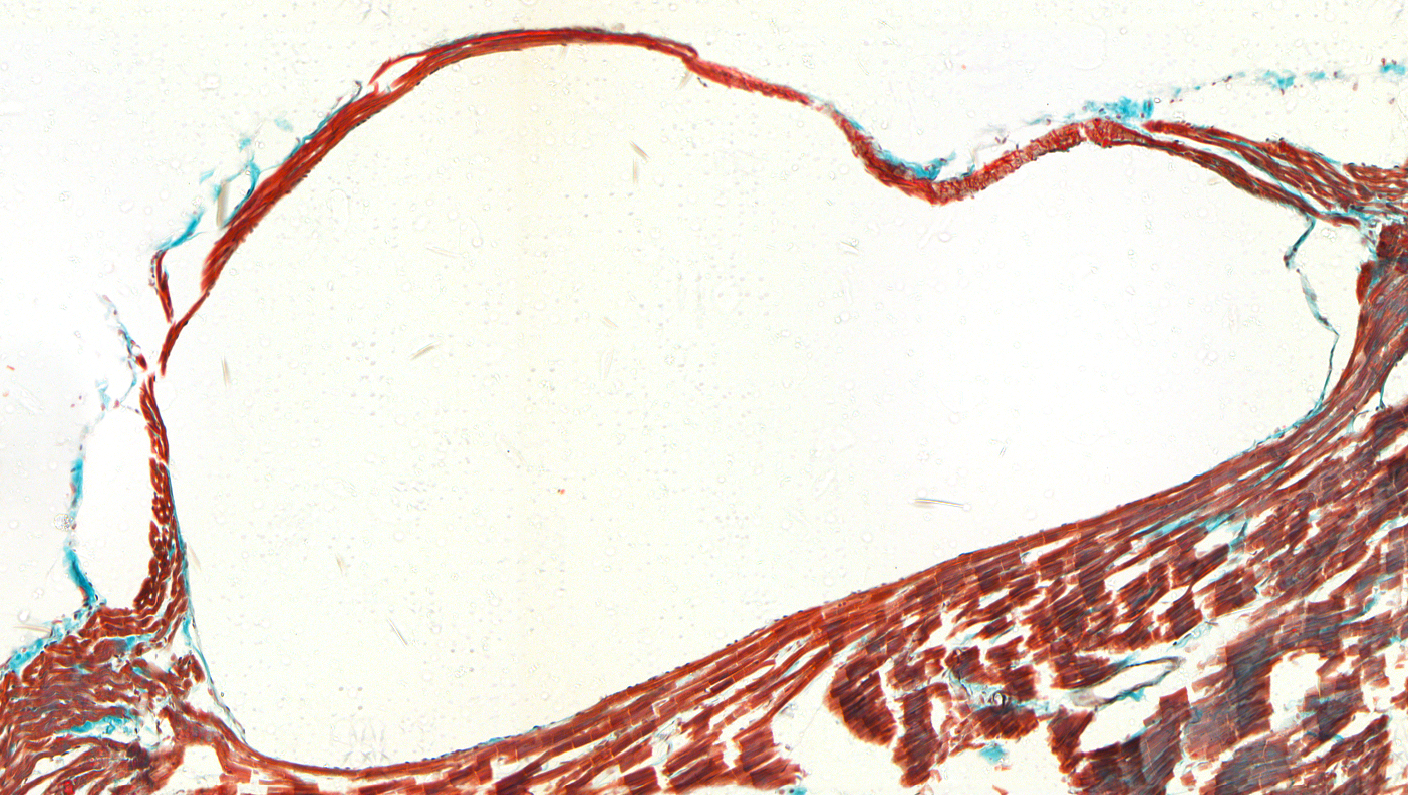
\includegraphics[width=1\textwidth]{Ch6/Figs/original_epicardial}}
        \subfigure[][Downsampled Slack1488.bmp]{
\includegraphics[width=1\textwidth]{Ch6/Figs/downsampled_epicardial}}
        \caption{Two histological images of an epicardial artery, one raw and one downsampled by a factor of 64.}
        \label{fig:downsampled_vessel}
      \end{figure}
      
      \begin{landscape}
        \begin{figure}[htbp]
          \centering
          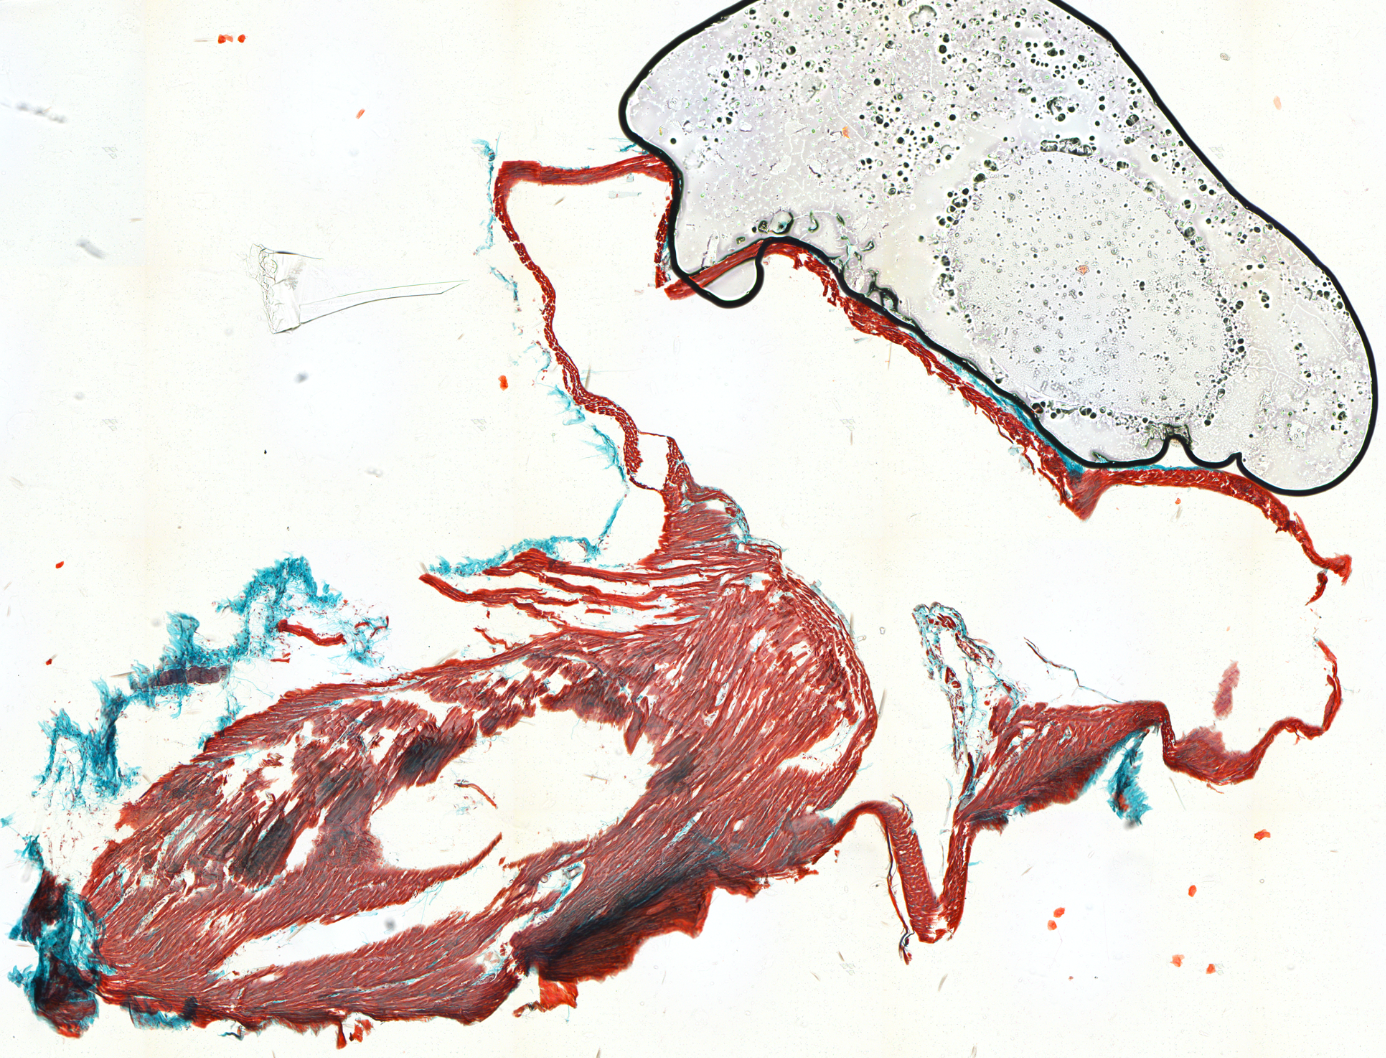
\includegraphics[width=1.3\textwidth]{Ch6/Figs/damaged_slice}
          \caption{A damaged slice close to the left extremity of the heart. The tissue is severely damaged and folded in place. There is also a large bubble trapped between the two imaging slides.}
          \label{fig:damaged_slice}
        \end{figure}
      \end{landscape}
      
    
    \subsubsection{Transforms} % (fold)
    \label{sub:transforms}
      The registration is achieved in two main stages. A rigid iteration of 3-D volume alignments and 2-D slice registrations is followed by a final 2-D Demons\cite{Yoo:2002p160} deformable registration of each with a 2-D MRI cross-section at the equivalent position. Figure~\ref{fig:algorithm} displays a graphical overview of the procedure. First, the downsampled histological images are stacked on top of each other, so that they share a common centre and orientation. The resulting volume is as wide as the widest image and as tall as the tallest, with black pixels to fill the spaces where each 2-D image is undefined. A `mask' is also generated, a binary image of the same dimensions as the volume stack, with value 1 within a histological slice, and zero otherwise. The mask is used by the metric to specify which pixels will be taken into consideration. The initial volume is displayed in Figure~\ref{fig:Seg3D_histology} and its associated mask in Figure~\ref{fig:Seg3D_mask}. The stack is then registered in 3-D against the segmented MRI data, to give an approximate alignment. 2-D images are extracted from the MRI volume where each of the histological slices lie, and the 2-D registration of the slices against these images brings them much closer into alignment with each other. With the new 2-D coordinates, a volume stack is again constructed and the loop repeats until convergence.
      
      Once a rigidly registered volume is obtained, a final non-rigid registration is applied in-plane to each histological slice independently, against each corresponding extracted MRI slice. The Demons algorithm used to perform the non-rigid registration assumes equal intensities between the two images, and so a histogram  matching is applied to the histology slices before execution.
            
      \begin{figure}[htbp]
        \centering
        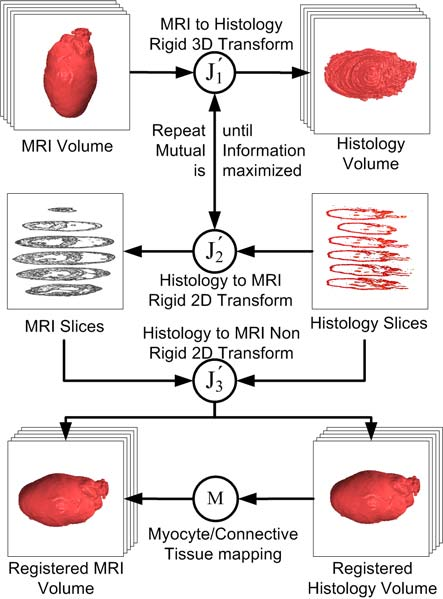
\includegraphics[width=0.8\textwidth]{Ch6/Figs/algorithm}
        \caption{A schematic of the registration algorithm from \cite{Mansoori:2007p221}. J$_1$ and J$_2$ are iterated between until the solution reaches a steady value. J$_3$ is then applied to each histology slice individually.}
        \label{fig:algorithm}
      \end{figure}

      \begin{landscape}
        \begin{figure}[htbp]
          \centering
          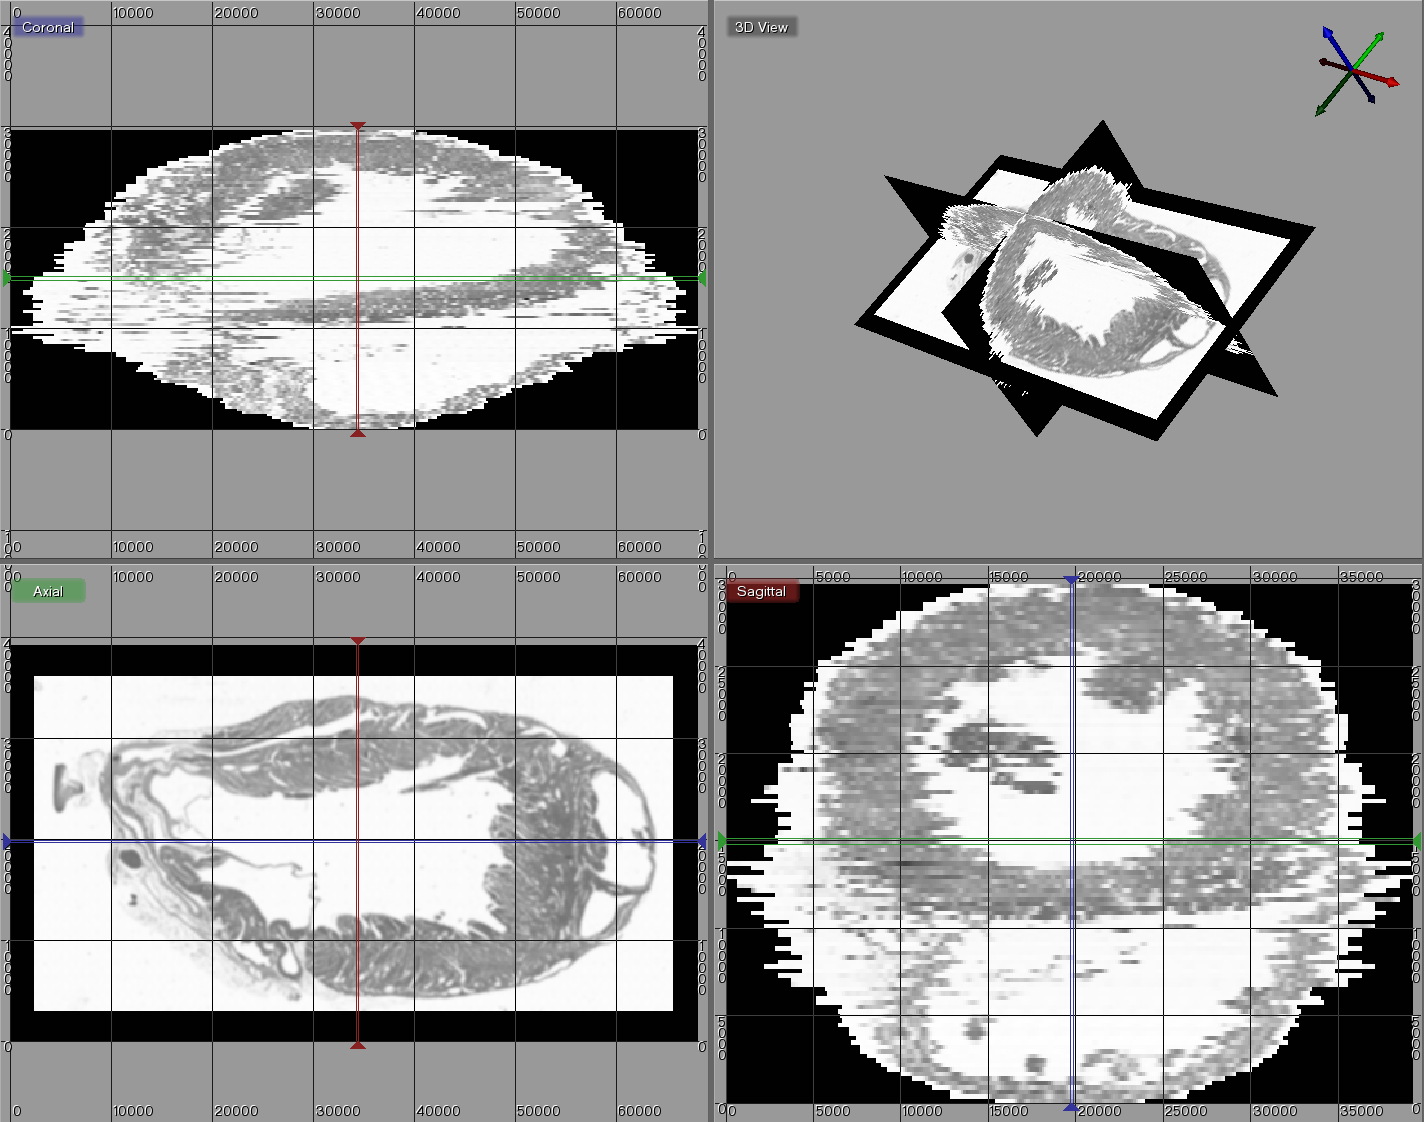
\includegraphics[width=1\textwidth]{Ch6/Figs/Seg3D_histology}
          \caption{The initial histology stack, visualised in the open source volume segmentation and visualisation tool Seg3D (www.sci.utah.edu/cibc/software/42-seg3d.html). Three perpendicular cross-sections through the volume are displayed in the top right and rendered flat in the remaining panels. The bottom left cross-section is in the plane of the histology slices and is in contrast with the misaligned, jagged appearance of the two planes perpendicular to the slices in the top left and bottom right. Notice the slice in the bottom left is centred and without rotation. Even before registration, the approximate form of the heart can be discerned. For example, note the two ventricles and a papillary muscle in the bottom right panel. Black pixels fill the undefined regions.}
          \label{fig:Seg3D_histology}
        \end{figure}
      \end{landscape}
      
      \begin{landscape}
        \begin{figure}[htbp]
          \centering
          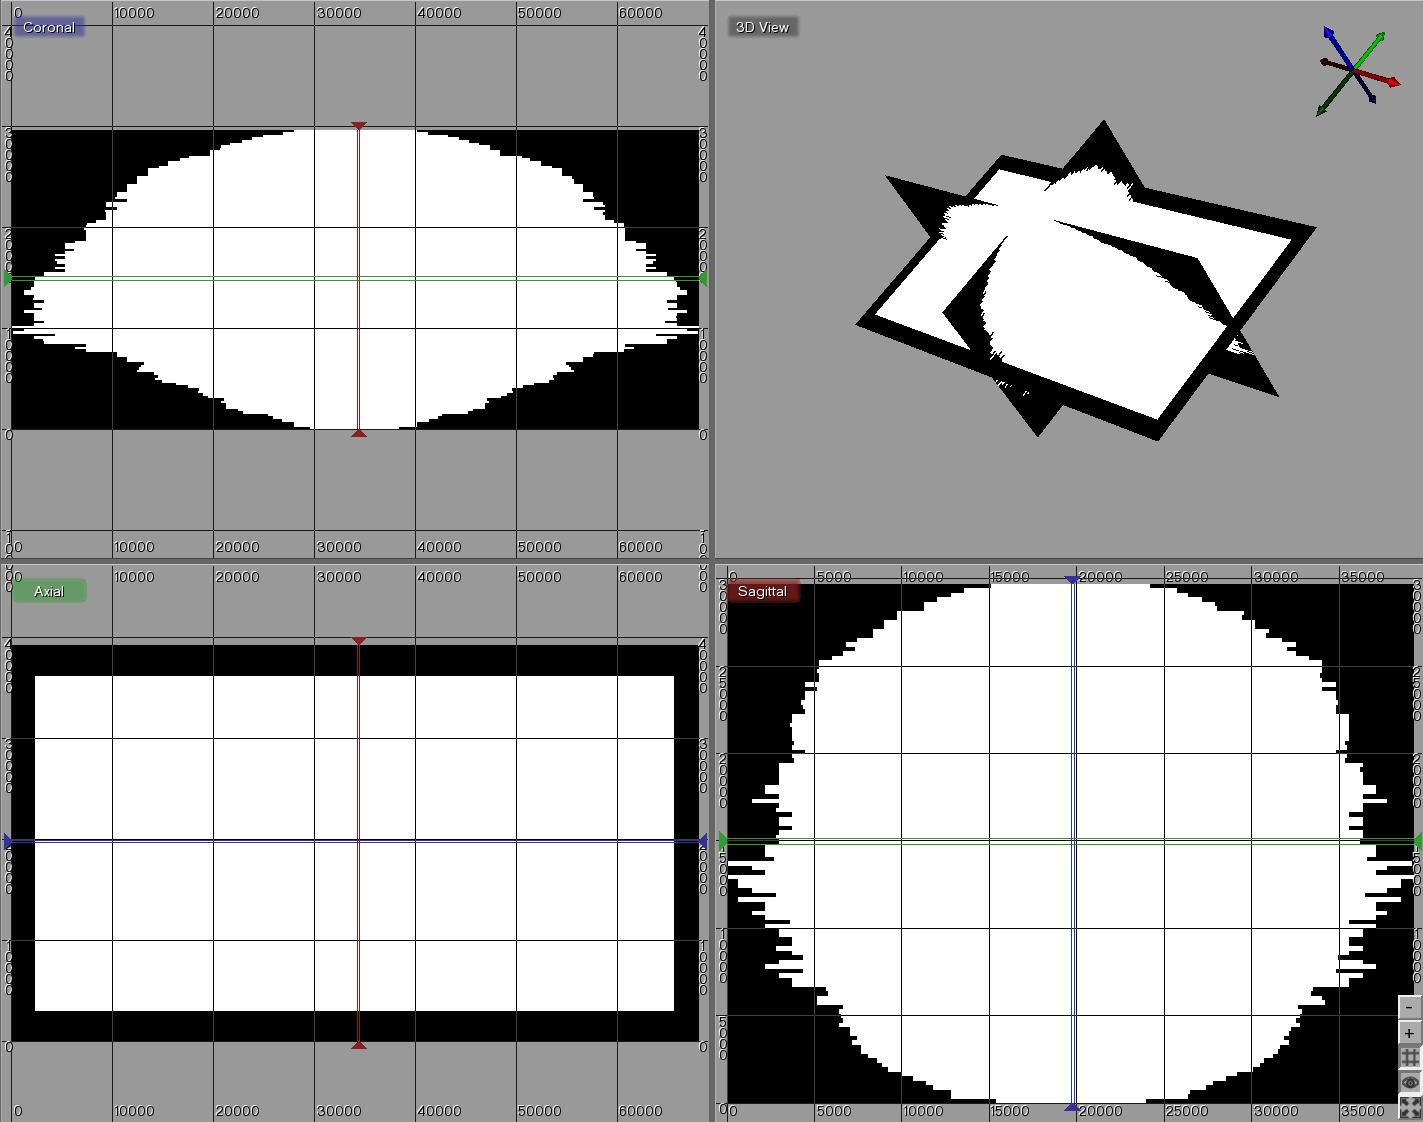
\includegraphics[width=1\textwidth]{Ch6/Figs/Seg3D_mask}
          \caption{The binary mask associated with the histological stack, from the same view as Figure~\ref{fig:Seg3D_histology}. Only the histology pixels that are white in the mask are used in the calculation of the mutual information metric.}
          \label{fig:Seg3D_mask}
        \end{figure}
      \end{landscape}
      
      \begin{landscape}
        \begin{figure}[htbp]
          \centering
          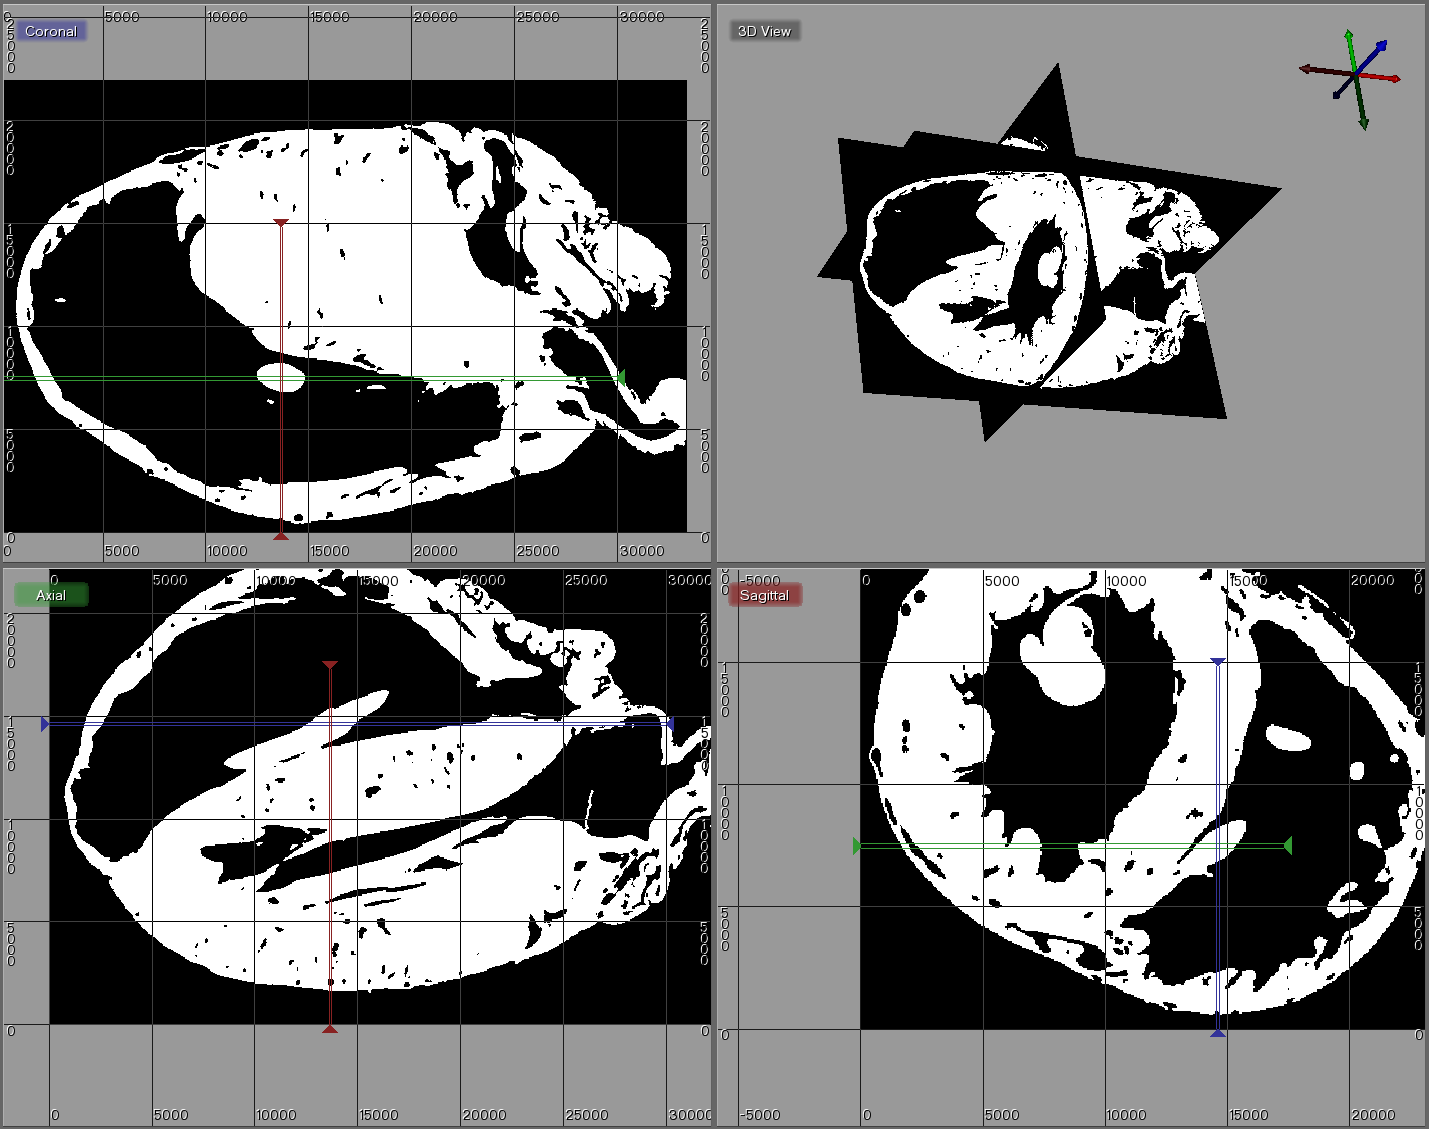
\includegraphics[width=1\textwidth]{Ch6/Figs/Seg3D_MRI}
          \caption{A segmentation of the raw MRI data from Bishop et al. \cite{Bishop:2009p444}. All three cross-sectional panels are aligned and coherent, with detailed anatomical features visible.}
          \label{fig:Seg3D_MRI}
        \end{figure}
      \end{landscape}
    
    
    \subsubsection{Interpolation} % (fold)
    \label{sub:interpolation}
      ITK provides four methods of interpolation: nearest neighbour, linear, B-spline and windowed sinc. Nearest neighbour interpolation simply returns the value of the closest pixel in the image being sampled. This requires the least amount of computation of the four methods, but results in a more jagged optimisation function, which could increase the time to convergence, the exact value converged upon, or in rare cases could prevent convergence to the global minimum. More accurately, but slightly more expensively, the value can be linearly interpolated from the four corners of the containing square or eight of the containing cube. Even more accurately, the image intensity can be calculated using B-spline basis functions. However, values may lie outside the range of input image intensities, causing saturation. Finally, the most accurate is the windowed sinc interpolator. Interpolation is based on the Fourier analysis of a sampled smooth spatial function. The pixel intensity is the result of a convolution of the sinc function with a window of neighbouring pixels. This requires by a stretch the most computation. For our purposes, linear interpolation provided the best compromise between efficiency and accuracy.
    
    \subsubsection{Metric} % (fold)
    \label{sub:metric}
      The metrics available in ITK compare the gray-scale intensity of two images to measure how well they are aligned. Masks can be set for both the fixed and moving images to restrict evaluation of the metric within a specified region. The choice of metric critically affects the shape of the optimisation function in the parameter space, and some are only suitable to compare images of the same modality. A mean squares metric requires that equivalent points in the two images are at the same intensity in order to function well. A normalised correlation metric is slightly more flexible in its range of application, but still assumes a linear relationship between equivalent intensities in the two images. A mutual information metric assumes no such relationship. The mutual information between two images is a measure of how much information a random intensity from one image confers about the intensity at the equivalent point in the other image. For example, a region could be uniquely dark grey in one image, but uniquely red in the other. Regardless of the colour or intensity, if a randomly selected pixel turns out to be that exact dark grey in the first image, one can be sure that the same point in the second image is red, and vice versa; mutual information is maximised. If for some reason, these regions were misaligned, that certainty is compromised, and the contribution to the mutual information coefficient from that region is reduced. The mutual information approach is ideally suited to the registration of MRI to histology, where the relationship between intensities is highly complex.
    
    
    \subsubsection{Optimisation} % (fold)
    \label{sub:optimisation}
      The optimiser iteratively moves through the space defined by the transform parameters from a set of initial coordinates, in an attempt to minimise the cost function evaluated by the metric. ITK provides a range of algorithms to achieve this task in the most efficient and reliable way possible. Throughout the registration process, a gradient descent optimiser was employed. This optimiser is a robust, general purpose algorithm that requires little configuration.
    
    
  \subsection{Discussion and Conclusions} % (fold)
  \label{sec:discussion_and_conclusions}
    There are three main reasons why the method described here is a strong approach to a difficult problem. Firstly, the approach is robust and likely to find the optimal solution. The mutual information metric is highly suitable for matching different modalities, the downsampling of the images acts to smooth out the optimised function and prevent trapping in local minima, and the optimisation algorithm is a good choice for an unknown topology. Completing rigid registration before releasing non-rigid degrees of freedom also helps ensure a good starting point in a high-dimensional non-rigid parameter space. Secondly, by dividing the optimisation into rigid and non-rigid components, and then again into 2-D and 3-D iterative steps, and thus greatly reducing the dimensionality of the parameter space at each step, the problem becomes computationally feasible. The downsampled data is also clearly very helpful in this regard, the results of which could be used to initialise another registration using data at a higher resolution. Thirdly, the technique analogues the sequence of transformations engendered by the experimental method. The orientation of the heart is altered when it is moved from the MRI machine into the histological apparatus, then the slices are translated, rotated and deformed between the surface of the block and the imaging slide. It is also worth noting that the non-rigid transform would be able to match unrelated MRI and histology slices, and so must be executed last to minimise any erroneous effects of this freedom.
    
    The presented algorithm does not correct for 3-D out-of-plane deformations, possibly resulting from the wax embedding process. Mansoori et al. \cite{Mansoori:2007p221} believe that these deformations have a negligible effect on the final result, but do not rule out the inclusion of a final 3-D deformable transform when registering other histology datasets.

TRANSFER THESIS
